\documentclass{beamer}
\usetheme{Warsaw}
\usecolortheme{dolphin}
\usepackage{amsmath}
\usepackage{amsfonts}
\usepackage{amssymb}
%\usepackage{CJKutf8}
\title{Introduction to Fourier Transform and Signal Analysis}
\author{\texorpdfstring{Zong-han, Xie\newline\url{icbm0926@gmail.com}}{Zong-han, Xie}}
\begin{document}
%\begin{CJK}{UTF8}{cwmc}
\begin{frame}
\titlepage
\end{frame}
\begin{frame}[label=licensepage]
\frametitle{License of this document}
Introduction to Fourier Transform and Signal Analysis by Zong-han, Xie (\href{icbm0926@gmail.com}{icbm0926@gmail.com}) is licensed under a Creative Commons Attribution-NonCommercial 4.0 International License. \newline
\begin{center}
\includegraphics[scale=1]{by-nc-sa.eps}
\end{center}
\end{frame}
\AtBeginSection[]
{
  \begin{frame}
    \frametitle{Outline}
    \tableofcontents[currentsection]
  \end{frame}
}
\section{Continuous Fourier Transform}
\begin{frame}
\frametitle{Orthogonal Condition}
\begin{itemize}
\item Any two vectors $\mathbf{a}$, $\mathbf{b}$ satisfied the following condition are mutually orthogonal. \newline
\begin{eqnarray}
\mathbf{a}^* \cdot \mathbf{b} = 0
\label{eq:ortho_vec}
\end{eqnarray}
\item Any two functions $f(x)$, $g(x)$ satisfied the following condition are mutually orthogonal. \newline
\begin{eqnarray}
\int{f^*(x)} \cdot {g(x)} dx = 0
\label{eq:ortho_func}
\end{eqnarray}
\item * means complex conjugate. \newline
\end{itemize}
\end{frame}
\begin{frame}
\frametitle{Fourier Series}
\begin{itemize}
\item $\cos nx $ and $\sin mx$ are mutually orthogonal in which n and m are integers.
\begin{eqnarray}
\int_{-\pi}^{\pi}{\cos nx} \cdot {\sin mx} dx = 0 \nonumber \\
\int_{-\pi}^{\pi}{\cos nx} \cdot {\cos mx} dx = \pi\delta_{nm} \nonumber \\
\int_{-\pi}^{\pi}{\sin nx} \cdot {\sin mx} dx = \pi\delta_{nm}
\end{eqnarray}
\item $\delta_{nm} $ is Dirac-delta symbol. It means $\delta_{nn} = 1$ and $\delta_{nm} = 0$ when $n \neq m$.
\end{itemize}
\end{frame}
\begin{frame}
\frametitle{Fourier Series}
\begin{itemize}
\item Since $\cos nx $ and $\sin mx$ are mutually orthogonal, we can expand an arbitrary function $f(x)$ with them. we shall have a series expansion.
\begin{eqnarray}
f(x)&=&a_0 + \sum_{k=1}^{\infty} \left(a_k\cos kx + b_k \sin kx\right) \nonumber \\
a_0&=&\frac{1}{2\pi}\int_{-\pi}^{\pi}f(x) dx \nonumber \\
a_k&=&\frac{1}{\pi}\int_{-\pi}^{\pi}f(x) \cos kx dx \nonumber \\
b_k&=&\frac{1}{\pi}\int_{-\pi}^{\pi}f(x) \sin kx dx
\label{eq:fseries}
\end{eqnarray}
\end{itemize}
\end{frame}
\section{From Continuous to Discrete Fourier Transform}
\begin{frame}

\end{frame}
\section{Calculate DFT with Python-numpy}
\begin{frame}

\end{frame}

%---------------Examples of Latex---------
\begin{frame}
\frametitle{2nd page}
\begin{block}{block}
\begin{eqnarray}
\frac{1}{2}
\end{eqnarray}
\end{block}
\begin{alertblock}{alertblock}
alertblock content
\end{alertblock}
\end{frame}
\begin{frame}
\frametitle{3rd page}
\begin{itemize}
\item<1-> 第一
\item<1-> 2nd
\item<2-> 3rd
\item<3-> etc.
\hyperlink{1stpage}{\beamerbutton{go fuck}}
\end{itemize}
\end{frame}
%\end{CJK}
\end{document}
